% !TEX program = pdflatex
% Falsifier? I just met her! -- CISC 7200 final, 14 May 2026
% metropolis structure with chrome stripped, lavender accent.

\documentclass[aspectratio=169]{beamer}

\ifdefined\OnlyNotes
  \setbeameroption{show only notes}
\else
  \ifdefined\WithNotes
    \setbeameroption{show notes}
  \fi
\fi

% theme.tex -- Crane-inspired beamer theme.
% Palatino body via mathpazo, metropolis structure with chrome stripped,
% lavender accent. Loaded by `% theme.tex -- Crane-inspired beamer theme.
% Palatino body via mathpazo, metropolis structure with chrome stripped,
% lavender accent. Loaded by `% theme.tex -- Crane-inspired beamer theme.
% Palatino body via mathpazo, metropolis structure with chrome stripped,
% lavender accent. Loaded by `\input{theme}` from slides.tex.

\usetheme[progressbar=none,
          numbering=none,
          block=fill,
          sectionpage=simple,
          titleformat title=regular,
          titleformat frame=regular,
          background=light]{metropolis}

%%% ----- Fonts -----
\usepackage[T1]{fontenc}
\usepackage[utf8]{inputenc}
\usepackage{mathpazo}
\linespread{1.06}

%%% ----- TikZ -----
\usepackage{tikz}
\usetikzlibrary{calc, decorations.pathmorphing, positioning, arrows.meta, fit, backgrounds, shapes.geometric}

%%% ----- Rounded box (used in print-friendly note pages) -----
\usepackage[skins]{tcolorbox}

%%% ----- Semantic palette -----
% primary       : main accent (title band, section divider, bullets, witness dots)
% primary_light : block backgrounds, secondary fill tint
% text          : body text, near-black
% mute          : muted gray for asides, subtitle, captions
% accent        : rare warm emphasis for refutation / alerted text
\definecolor{color_primary}{HTML}{C3C4E3}
\definecolor{color_primary_light}{HTML}{E4E5F2}
\definecolor{color_text}{HTML}{1A1A1A}
\definecolor{color_mute}{HTML}{6E6E78}
\definecolor{color_accent}{HTML}{8C1D40}

\setbeamercolor{normal text}{fg=color_text, bg=white}
\setbeamercolor{frametitle}{fg=color_text, bg=white}
\setbeamercolor{title}{fg=color_text}
\setbeamercolor{subtitle}{fg=color_mute}
\setbeamercolor{author}{fg=color_text}
\setbeamercolor{date}{fg=color_mute}
\setbeamercolor{section title}{fg=color_text}
\setbeamercolor{progress bar}{fg=color_primary}
\setbeamercolor{title separator}{fg=color_primary}
\setbeamercolor{background canvas}{bg=white}
\setbeamercolor{alerted text}{fg=color_accent}
\setbeamercolor{block title}{fg=color_text, bg=color_primary_light}
\setbeamercolor{block body}{fg=color_text, bg=color_primary_light}

%%% ----- Serif body, italic titles -----
\usefonttheme{serif}
\setbeamerfont{frametitle}{family=\rmfamily, shape=\itshape, series=\mdseries, size=\Large}
\setbeamerfont{title}{family=\rmfamily, shape=\itshape, series=\mdseries, size=\Huge}
\setbeamerfont{subtitle}{family=\rmfamily, shape=\itshape, size=\large}
\setbeamerfont{author}{family=\rmfamily, shape=\upshape}
\setbeamerfont{date}{family=\rmfamily, shape=\upshape, size=\small}
\setbeamerfont{section title}{family=\rmfamily, shape=\itshape, size=\Huge}
\setbeamerfont{block title}{family=\rmfamily, shape=\itshape, series=\mdseries}
\setbeamerfont{itemize/enumerate body}{size=\normalsize}
\setbeamerfont{itemize/enumerate subbody}{size=\small}

% Bullets: thin, primary
\setbeamertemplate{itemize item}{\textcolor{color_primary}{\rule[0.25ex]{0.5em}{0.5pt}}}
\setbeamertemplate{itemize subitem}{\textcolor{color_mute}{\textendash}}
\setbeamertemplate{itemize subsubitem}{\textcolor{color_mute}{$\cdot$}}

%%% ----- Print-friendly mode -----
% When building notes outputs (\WithNotes or \OnlyNotes), drop full-page
% color fills in favor of rounded inset borders, and resize the output
% paper to US Letter (landscape) so the deck prints on standard paper.
% Slides projector build keeps the native 16:9 paper.
\newif\ifprintfriendly
\ifdefined\WithNotes\printfriendlytrue\fi
\ifdefined\OnlyNotes\printfriendlytrue\fi

\ifprintfriendly
  \usepackage{pgfpages}
  \pgfpagesuselayout{resize to}[letterpaper, landscape]
\fi

\ifprintfriendly
  % Section divider: rounded inset border, italic name centered.
  \setbeamertemplate{section page}{%
    \begin{tikzpicture}[remember picture, overlay]
      \draw[color_primary, line width=0.8pt, rounded corners=10pt]
        ([xshift=1.0cm, yshift=-1.0cm]current page.north west)
        rectangle
        ([xshift=-1.0cm, yshift=1.0cm]current page.south east);
    \end{tikzpicture}%
    \vfill
    \begin{center}
      {\usebeamerfont{section title}\itshape\insertsectionhead}
    \end{center}
    \vfill
  }

  % Title page: no top band, plain typography.
  \setbeamertemplate{title page}{%
    \vspace*{2.4cm}
    \begin{minipage}[t]{\textwidth}
      \raggedright
      {\usebeamerfont{title}\usebeamercolor[fg]{title}\inserttitle}\par\vspace{0.35em}
      {\usebeamerfont{subtitle}\usebeamercolor[fg]{subtitle}\insertsubtitle}\par
    \end{minipage}
    \vspace{1.8cm}
    \begin{minipage}{\textwidth}
      \raggedright
      {\usebeamerfont{author}\usebeamercolor[fg]{author}\insertauthor}\par\vspace{0.15em}
      {\usebeamerfont{date}\usebeamercolor[fg]{date}\insertdate}\par
    \end{minipage}
  }

  % Note pages: white background, rounded inset border, thumbnail top-right,
  % heading top-left, notes flow below. No default gray strips.
  \setbeamercolor{note page}{fg=color_text, bg=white}
  \setbeamercolor{note title}{fg=color_text, bg=white}
  \setbeamercolor{note date}{fg=color_mute, bg=white}
  % Rounded inset border via tcolorbox. Robust in both `show notes`
  % (interleaved) and `show only notes` (notes-only) builds.
  \setbeamertemplate{note page}{%
    \begin{tcolorbox}[
      enhanced, arc=8pt, boxrule=0.6pt,
      colback=white, colframe=color_primary,
      left=12pt, right=12pt, top=6pt, bottom=6pt,
      width=\dimexpr\paperwidth-1.2cm\relax,
      before=\hspace*{0.6cm}, after=\hspace*{0.6cm}\par
    ]
      \hfill\insertslideintonotes{0.3}\par
      \vspace{0.3cm}\par
      \footnotesize\insertnote
    \end{tcolorbox}%
  }
\else
  % Full-bleed section divider (projection)
  \setbeamertemplate{section page}{%
    \begin{tikzpicture}[remember picture, overlay]
      \fill[color_primary] (current page.south west) rectangle (current page.north east);
    \end{tikzpicture}%
    \vfill
    \begin{center}
      {\usebeamerfont{section title}\itshape\insertsectionhead}
    \end{center}
    \vfill
  }

  % Title page: primary top band, italic title, simple (projection)
  \setbeamertemplate{title page}{%
    \begin{tikzpicture}[remember picture, overlay]
      \fill[color_primary] (current page.north west) rectangle ([yshift=-3.6cm]current page.north east);
    \end{tikzpicture}%
    \vspace*{0.6cm}
    \begin{minipage}[t]{\textwidth}
      \raggedright
      {\usebeamerfont{title}\usebeamercolor[fg]{title}\inserttitle}\par\vspace{0.35em}
      {\usebeamerfont{subtitle}\usebeamercolor[fg]{subtitle}\insertsubtitle}\par
    \end{minipage}
    \vspace{2.0cm}
    \begin{minipage}{\textwidth}
      \raggedright
      {\usebeamerfont{author}\usebeamercolor[fg]{author}\insertauthor}\par\vspace{0.15em}
      {\usebeamerfont{date}\usebeamercolor[fg]{date}\insertdate}\par
    \end{minipage}
  }
\fi

%%% ----- TikZ styles -----
\tikzset{
  space_blob/.style={draw=color_mute, line width=0.7pt, rounded corners=10pt, fill=white},
  space_divide/.style={draw=color_mute, line width=0.7pt, decorate, decoration={random steps, segment length=8pt, amplitude=2.5pt}},
  figure_label/.style={font=\rmfamily\itshape, text=color_text},
  figure_dot/.style={circle, fill=color_text, inner sep=0pt, minimum size=4pt},
  witness_dot/.style={circle, fill=color_primary, draw=color_text, line width=0.4pt, inner sep=0pt, minimum size=5pt},
  refutation_dot/.style={circle, fill=color_accent, draw=color_accent, inner sep=0pt, minimum size=5pt},
  diagram_node/.style={font=\rmfamily, text=color_text, inner sep=4pt},
  diagram_arrow/.style={-{Stealth[length=4pt, width=4pt]}, draw=color_text, line width=0.6pt},
}
` from slides.tex.

\usetheme[progressbar=none,
          numbering=none,
          block=fill,
          sectionpage=simple,
          titleformat title=regular,
          titleformat frame=regular,
          background=light]{metropolis}

%%% ----- Fonts -----
\usepackage[T1]{fontenc}
\usepackage[utf8]{inputenc}
\usepackage{mathpazo}
\linespread{1.06}

%%% ----- TikZ -----
\usepackage{tikz}
\usetikzlibrary{calc, decorations.pathmorphing, positioning, arrows.meta, fit, backgrounds, shapes.geometric}

%%% ----- Rounded box (used in print-friendly note pages) -----
\usepackage[skins]{tcolorbox}

%%% ----- Semantic palette -----
% primary       : main accent (title band, section divider, bullets, witness dots)
% primary_light : block backgrounds, secondary fill tint
% text          : body text, near-black
% mute          : muted gray for asides, subtitle, captions
% accent        : rare warm emphasis for refutation / alerted text
\definecolor{color_primary}{HTML}{C3C4E3}
\definecolor{color_primary_light}{HTML}{E4E5F2}
\definecolor{color_text}{HTML}{1A1A1A}
\definecolor{color_mute}{HTML}{6E6E78}
\definecolor{color_accent}{HTML}{8C1D40}

\setbeamercolor{normal text}{fg=color_text, bg=white}
\setbeamercolor{frametitle}{fg=color_text, bg=white}
\setbeamercolor{title}{fg=color_text}
\setbeamercolor{subtitle}{fg=color_mute}
\setbeamercolor{author}{fg=color_text}
\setbeamercolor{date}{fg=color_mute}
\setbeamercolor{section title}{fg=color_text}
\setbeamercolor{progress bar}{fg=color_primary}
\setbeamercolor{title separator}{fg=color_primary}
\setbeamercolor{background canvas}{bg=white}
\setbeamercolor{alerted text}{fg=color_accent}
\setbeamercolor{block title}{fg=color_text, bg=color_primary_light}
\setbeamercolor{block body}{fg=color_text, bg=color_primary_light}

%%% ----- Serif body, italic titles -----
\usefonttheme{serif}
\setbeamerfont{frametitle}{family=\rmfamily, shape=\itshape, series=\mdseries, size=\Large}
\setbeamerfont{title}{family=\rmfamily, shape=\itshape, series=\mdseries, size=\Huge}
\setbeamerfont{subtitle}{family=\rmfamily, shape=\itshape, size=\large}
\setbeamerfont{author}{family=\rmfamily, shape=\upshape}
\setbeamerfont{date}{family=\rmfamily, shape=\upshape, size=\small}
\setbeamerfont{section title}{family=\rmfamily, shape=\itshape, size=\Huge}
\setbeamerfont{block title}{family=\rmfamily, shape=\itshape, series=\mdseries}
\setbeamerfont{itemize/enumerate body}{size=\normalsize}
\setbeamerfont{itemize/enumerate subbody}{size=\small}

% Bullets: thin, primary
\setbeamertemplate{itemize item}{\textcolor{color_primary}{\rule[0.25ex]{0.5em}{0.5pt}}}
\setbeamertemplate{itemize subitem}{\textcolor{color_mute}{\textendash}}
\setbeamertemplate{itemize subsubitem}{\textcolor{color_mute}{$\cdot$}}

%%% ----- Print-friendly mode -----
% When building notes outputs (\WithNotes or \OnlyNotes), drop full-page
% color fills in favor of rounded inset borders, and resize the output
% paper to US Letter (landscape) so the deck prints on standard paper.
% Slides projector build keeps the native 16:9 paper.
\newif\ifprintfriendly
\ifdefined\WithNotes\printfriendlytrue\fi
\ifdefined\OnlyNotes\printfriendlytrue\fi

\ifprintfriendly
  \usepackage{pgfpages}
  \pgfpagesuselayout{resize to}[letterpaper, landscape]
\fi

\ifprintfriendly
  % Section divider: rounded inset border, italic name centered.
  \setbeamertemplate{section page}{%
    \begin{tikzpicture}[remember picture, overlay]
      \draw[color_primary, line width=0.8pt, rounded corners=10pt]
        ([xshift=1.0cm, yshift=-1.0cm]current page.north west)
        rectangle
        ([xshift=-1.0cm, yshift=1.0cm]current page.south east);
    \end{tikzpicture}%
    \vfill
    \begin{center}
      {\usebeamerfont{section title}\itshape\insertsectionhead}
    \end{center}
    \vfill
  }

  % Title page: no top band, plain typography.
  \setbeamertemplate{title page}{%
    \vspace*{2.4cm}
    \begin{minipage}[t]{\textwidth}
      \raggedright
      {\usebeamerfont{title}\usebeamercolor[fg]{title}\inserttitle}\par\vspace{0.35em}
      {\usebeamerfont{subtitle}\usebeamercolor[fg]{subtitle}\insertsubtitle}\par
    \end{minipage}
    \vspace{1.8cm}
    \begin{minipage}{\textwidth}
      \raggedright
      {\usebeamerfont{author}\usebeamercolor[fg]{author}\insertauthor}\par\vspace{0.15em}
      {\usebeamerfont{date}\usebeamercolor[fg]{date}\insertdate}\par
    \end{minipage}
  }

  % Note pages: white background, rounded inset border, thumbnail top-right,
  % heading top-left, notes flow below. No default gray strips.
  \setbeamercolor{note page}{fg=color_text, bg=white}
  \setbeamercolor{note title}{fg=color_text, bg=white}
  \setbeamercolor{note date}{fg=color_mute, bg=white}
  % Rounded inset border via tcolorbox. Robust in both `show notes`
  % (interleaved) and `show only notes` (notes-only) builds.
  \setbeamertemplate{note page}{%
    \begin{tcolorbox}[
      enhanced, arc=8pt, boxrule=0.6pt,
      colback=white, colframe=color_primary,
      left=12pt, right=12pt, top=6pt, bottom=6pt,
      width=\dimexpr\paperwidth-1.2cm\relax,
      before=\hspace*{0.6cm}, after=\hspace*{0.6cm}\par
    ]
      \hfill\insertslideintonotes{0.3}\par
      \vspace{0.3cm}\par
      \footnotesize\insertnote
    \end{tcolorbox}%
  }
\else
  % Full-bleed section divider (projection)
  \setbeamertemplate{section page}{%
    \begin{tikzpicture}[remember picture, overlay]
      \fill[color_primary] (current page.south west) rectangle (current page.north east);
    \end{tikzpicture}%
    \vfill
    \begin{center}
      {\usebeamerfont{section title}\itshape\insertsectionhead}
    \end{center}
    \vfill
  }

  % Title page: primary top band, italic title, simple (projection)
  \setbeamertemplate{title page}{%
    \begin{tikzpicture}[remember picture, overlay]
      \fill[color_primary] (current page.north west) rectangle ([yshift=-3.6cm]current page.north east);
    \end{tikzpicture}%
    \vspace*{0.6cm}
    \begin{minipage}[t]{\textwidth}
      \raggedright
      {\usebeamerfont{title}\usebeamercolor[fg]{title}\inserttitle}\par\vspace{0.35em}
      {\usebeamerfont{subtitle}\usebeamercolor[fg]{subtitle}\insertsubtitle}\par
    \end{minipage}
    \vspace{2.0cm}
    \begin{minipage}{\textwidth}
      \raggedright
      {\usebeamerfont{author}\usebeamercolor[fg]{author}\insertauthor}\par\vspace{0.15em}
      {\usebeamerfont{date}\usebeamercolor[fg]{date}\insertdate}\par
    \end{minipage}
  }
\fi

%%% ----- TikZ styles -----
\tikzset{
  space_blob/.style={draw=color_mute, line width=0.7pt, rounded corners=10pt, fill=white},
  space_divide/.style={draw=color_mute, line width=0.7pt, decorate, decoration={random steps, segment length=8pt, amplitude=2.5pt}},
  figure_label/.style={font=\rmfamily\itshape, text=color_text},
  figure_dot/.style={circle, fill=color_text, inner sep=0pt, minimum size=4pt},
  witness_dot/.style={circle, fill=color_primary, draw=color_text, line width=0.4pt, inner sep=0pt, minimum size=5pt},
  refutation_dot/.style={circle, fill=color_accent, draw=color_accent, inner sep=0pt, minimum size=5pt},
  diagram_node/.style={font=\rmfamily, text=color_text, inner sep=4pt},
  diagram_arrow/.style={-{Stealth[length=4pt, width=4pt]}, draw=color_text, line width=0.6pt},
}
` from slides.tex.

\usetheme[progressbar=none,
          numbering=none,
          block=fill,
          sectionpage=simple,
          titleformat title=regular,
          titleformat frame=regular,
          background=light]{metropolis}

%%% ----- Fonts -----
\usepackage[T1]{fontenc}
\usepackage[utf8]{inputenc}
\usepackage{mathpazo}
\linespread{1.06}

%%% ----- TikZ -----
\usepackage{tikz}
\usetikzlibrary{calc, decorations.pathmorphing, positioning, arrows.meta, fit, backgrounds, shapes.geometric}

%%% ----- Rounded box (used in print-friendly note pages) -----
\usepackage[skins]{tcolorbox}

%%% ----- Semantic palette -----
% primary       : main accent (title band, section divider, bullets, witness dots)
% primary_light : block backgrounds, secondary fill tint
% text          : body text, near-black
% mute          : muted gray for asides, subtitle, captions
% accent        : rare warm emphasis for refutation / alerted text
\definecolor{color_primary}{HTML}{C3C4E3}
\definecolor{color_primary_light}{HTML}{E4E5F2}
\definecolor{color_text}{HTML}{1A1A1A}
\definecolor{color_mute}{HTML}{6E6E78}
\definecolor{color_accent}{HTML}{8C1D40}

\setbeamercolor{normal text}{fg=color_text, bg=white}
\setbeamercolor{frametitle}{fg=color_text, bg=white}
\setbeamercolor{title}{fg=color_text}
\setbeamercolor{subtitle}{fg=color_mute}
\setbeamercolor{author}{fg=color_text}
\setbeamercolor{date}{fg=color_mute}
\setbeamercolor{section title}{fg=color_text}
\setbeamercolor{progress bar}{fg=color_primary}
\setbeamercolor{title separator}{fg=color_primary}
\setbeamercolor{background canvas}{bg=white}
\setbeamercolor{alerted text}{fg=color_accent}
\setbeamercolor{block title}{fg=color_text, bg=color_primary_light}
\setbeamercolor{block body}{fg=color_text, bg=color_primary_light}

%%% ----- Serif body, italic titles -----
\usefonttheme{serif}
\setbeamerfont{frametitle}{family=\rmfamily, shape=\itshape, series=\mdseries, size=\Large}
\setbeamerfont{title}{family=\rmfamily, shape=\itshape, series=\mdseries, size=\Huge}
\setbeamerfont{subtitle}{family=\rmfamily, shape=\itshape, size=\large}
\setbeamerfont{author}{family=\rmfamily, shape=\upshape}
\setbeamerfont{date}{family=\rmfamily, shape=\upshape, size=\small}
\setbeamerfont{section title}{family=\rmfamily, shape=\itshape, size=\Huge}
\setbeamerfont{block title}{family=\rmfamily, shape=\itshape, series=\mdseries}
\setbeamerfont{itemize/enumerate body}{size=\normalsize}
\setbeamerfont{itemize/enumerate subbody}{size=\small}

% Bullets: thin, primary
\setbeamertemplate{itemize item}{\textcolor{color_primary}{\rule[0.25ex]{0.5em}{0.5pt}}}
\setbeamertemplate{itemize subitem}{\textcolor{color_mute}{\textendash}}
\setbeamertemplate{itemize subsubitem}{\textcolor{color_mute}{$\cdot$}}

%%% ----- Print-friendly mode -----
% When building notes outputs (\WithNotes or \OnlyNotes), drop full-page
% color fills in favor of rounded inset borders, and resize the output
% paper to US Letter (landscape) so the deck prints on standard paper.
% Slides projector build keeps the native 16:9 paper.
\newif\ifprintfriendly
\ifdefined\WithNotes\printfriendlytrue\fi
\ifdefined\OnlyNotes\printfriendlytrue\fi

\ifprintfriendly
  \usepackage{pgfpages}
  \pgfpagesuselayout{resize to}[letterpaper, landscape]
\fi

\ifprintfriendly
  % Section divider: rounded inset border, italic name centered.
  \setbeamertemplate{section page}{%
    \begin{tikzpicture}[remember picture, overlay]
      \draw[color_primary, line width=0.8pt, rounded corners=10pt]
        ([xshift=1.0cm, yshift=-1.0cm]current page.north west)
        rectangle
        ([xshift=-1.0cm, yshift=1.0cm]current page.south east);
    \end{tikzpicture}%
    \vfill
    \begin{center}
      {\usebeamerfont{section title}\itshape\insertsectionhead}
    \end{center}
    \vfill
  }

  % Title page: no top band, plain typography.
  \setbeamertemplate{title page}{%
    \vspace*{2.4cm}
    \begin{minipage}[t]{\textwidth}
      \raggedright
      {\usebeamerfont{title}\usebeamercolor[fg]{title}\inserttitle}\par\vspace{0.35em}
      {\usebeamerfont{subtitle}\usebeamercolor[fg]{subtitle}\insertsubtitle}\par
    \end{minipage}
    \vspace{1.8cm}
    \begin{minipage}{\textwidth}
      \raggedright
      {\usebeamerfont{author}\usebeamercolor[fg]{author}\insertauthor}\par\vspace{0.15em}
      {\usebeamerfont{date}\usebeamercolor[fg]{date}\insertdate}\par
    \end{minipage}
  }

  % Note pages: white background, rounded inset border, thumbnail top-right,
  % heading top-left, notes flow below. No default gray strips.
  \setbeamercolor{note page}{fg=color_text, bg=white}
  \setbeamercolor{note title}{fg=color_text, bg=white}
  \setbeamercolor{note date}{fg=color_mute, bg=white}
  % Rounded inset border via tcolorbox. Robust in both `show notes`
  % (interleaved) and `show only notes` (notes-only) builds.
  \setbeamertemplate{note page}{%
    \begin{tcolorbox}[
      enhanced, arc=8pt, boxrule=0.6pt,
      colback=white, colframe=color_primary,
      left=12pt, right=12pt, top=6pt, bottom=6pt,
      width=\dimexpr\paperwidth-1.2cm\relax,
      before=\hspace*{0.6cm}, after=\hspace*{0.6cm}\par
    ]
      \hfill\insertslideintonotes{0.3}\par
      \vspace{0.3cm}\par
      \footnotesize\insertnote
    \end{tcolorbox}%
  }
\else
  % Full-bleed section divider (projection)
  \setbeamertemplate{section page}{%
    \begin{tikzpicture}[remember picture, overlay]
      \fill[color_primary] (current page.south west) rectangle (current page.north east);
    \end{tikzpicture}%
    \vfill
    \begin{center}
      {\usebeamerfont{section title}\itshape\insertsectionhead}
    \end{center}
    \vfill
  }

  % Title page: primary top band, italic title, simple (projection)
  \setbeamertemplate{title page}{%
    \begin{tikzpicture}[remember picture, overlay]
      \fill[color_primary] (current page.north west) rectangle ([yshift=-3.6cm]current page.north east);
    \end{tikzpicture}%
    \vspace*{0.6cm}
    \begin{minipage}[t]{\textwidth}
      \raggedright
      {\usebeamerfont{title}\usebeamercolor[fg]{title}\inserttitle}\par\vspace{0.35em}
      {\usebeamerfont{subtitle}\usebeamercolor[fg]{subtitle}\insertsubtitle}\par
    \end{minipage}
    \vspace{2.0cm}
    \begin{minipage}{\textwidth}
      \raggedright
      {\usebeamerfont{author}\usebeamercolor[fg]{author}\insertauthor}\par\vspace{0.15em}
      {\usebeamerfont{date}\usebeamercolor[fg]{date}\insertdate}\par
    \end{minipage}
  }
\fi

%%% ----- TikZ styles -----
\tikzset{
  space_blob/.style={draw=color_mute, line width=0.7pt, rounded corners=10pt, fill=white},
  space_divide/.style={draw=color_mute, line width=0.7pt, decorate, decoration={random steps, segment length=8pt, amplitude=2.5pt}},
  figure_label/.style={font=\rmfamily\itshape, text=color_text},
  figure_dot/.style={circle, fill=color_text, inner sep=0pt, minimum size=4pt},
  witness_dot/.style={circle, fill=color_primary, draw=color_text, line width=0.4pt, inner sep=0pt, minimum size=5pt},
  refutation_dot/.style={circle, fill=color_accent, draw=color_accent, inner sep=0pt, minimum size=5pt},
  diagram_node/.style={font=\rmfamily, text=color_text, inner sep=4pt},
  diagram_arrow/.style={-{Stealth[length=4pt, width=4pt]}, draw=color_text, line width=0.6pt},
}


\usepackage{amsmath,amssymb,amsthm}

%%% ----- Math helpers -----
\newcommand{\IS}{I_{S}}
\newcommand{\N}{\mathbb{N}}
\newcommand{\re}{\textsl{r.e.}}

\title{Falsifier? I just met her!}
\subtitle{CISC 7200 final}
\author{David Souther}
\date{14 May 2026}

\begin{document}

%%% ============================================================
%%% I. OPENING
%%% ============================================================

\begin{frame}[plain,noframenumbering]
  \titlepage
\end{frame}
\note{%
  In this talk, we're going to talk about ``falsification''. You've just come across someone who's made a boast, or some claim about the world we live in. Do you believe them? Should you believe them? How would you decide when to believe them?

  Our friend Shapiro, and his colleagues Karl Popper and many others, have given us a very straightforward way, a mathematically provable way, to make that call.
}

\begin{frame}{Overview}
  \begin{itemize}
    \item When do you actually believe someone?
    \item Rice--Shapiro: one counterexample is enough to discredit
    \item What can a working software engineer do with that?
  \end{itemize}
\end{frame}
\note{%
  We'll start by re-treading Rice and Rice--Shapiro, just to stay on firm mathematical ground with proofs and everything. Then we'll throw that away to talk about what it means for philosophy and trusting people you talk to.

  Popper says the same thing as Shapiro, though in more words than symbols. We'll get into him in depth later, but Popper's main claim is that if you want to do science, if you want to really know the world, your description has to be clear enough that I have a chance to refute it.

  And at the end of this, I'm going to bring it back to my field, software engineering, and ostensibly Computer Science as well, and talk about how we can use these ideas to really ensure we're engineering the best software we can. Because every computer program is, actually, a proof of some theorem.
}

\begin{frame}{Roadmap}
  \begin{itemize}
    \item \emph{Theorems.} Rice and Rice--Shapiro
    \item \emph{History.} Archimedes, Newton, Popper
    \item \emph{Practice.} Tests and types
  \end{itemize}
\end{frame}
\note{%
  So that's the big picture. Here's a roadmap of how we'll get there. We're going to start with those theorems, like I said. The bulk of the talk is going to be an extended trip through history, checking in mainly with Archimedes, Newton, and this gentleman who might be a bit newer to you named Popper, and we'll see a few other friends along the way. Then we'll end with how Unit Testing and Typed Programming Languages give structure to those of us who practice software engineering.
}

%%% ============================================================
%%% II. THEOREMS
%%% ============================================================

\section{Theorems}

\begin{frame}{Setup}
  \begin{itemize}
    \item $S$, a set of partial computable functions
    \item $\IS$, its index set
    \item \emph{Trivial:} $S = \N$ or $S = \emptyset$
    \item \emph{Non-trivial:} every other partition
  \end{itemize}
  \vfill
  {\small\itshape\color{color_mute}
   $\IS$ asks of a function whether it has the property, not of a number whether it satisfies one.}
\end{frame}
\note{%
  Let's do a bit of setup. We start with $S$, a set of partial computable functions. Partial computable means that we're sure some natural numbers as inputs to this function will end with a value coming out, but we're not sure which ones.

  We have an index set $\IS$ of that set $S$, so we can assign a number to each function in $S$. We're not talking about the concrete case of the properties of any single number in any single function, but rather a class of functions as a black box. If $S$ is ``functions that calculate whether an input number is even'', any particular function might be testable with 0, 1, 2, 5, and 8 and we'd be OK with it. But we want to say, of \emph{any} function: is it a function that figures out if a given value is even?

  $S$ is the kinds of functions we want to identify, $\IS$ is a way to check if some function is in $S$. A couple points for completeness: $S$ is ``trivial'' if it's empty (no functions have this property, like ``the function is an elephant'') or if it's every function. Every function is a function, ok, yes, that's true thank you.
}

%%%---- Rice's theorem
\begin{frame}{Rice's theorem}
  \begin{block}{}
    If $S$ is non-trivial, then $\IS$ is undecidable.
  \end{block}
  \vskip 0.7em
  No general decision procedure can answer ``is this function in $S$?''
\end{frame}

\begin{frame}{Rice's theorem, drawn}
  \centering
  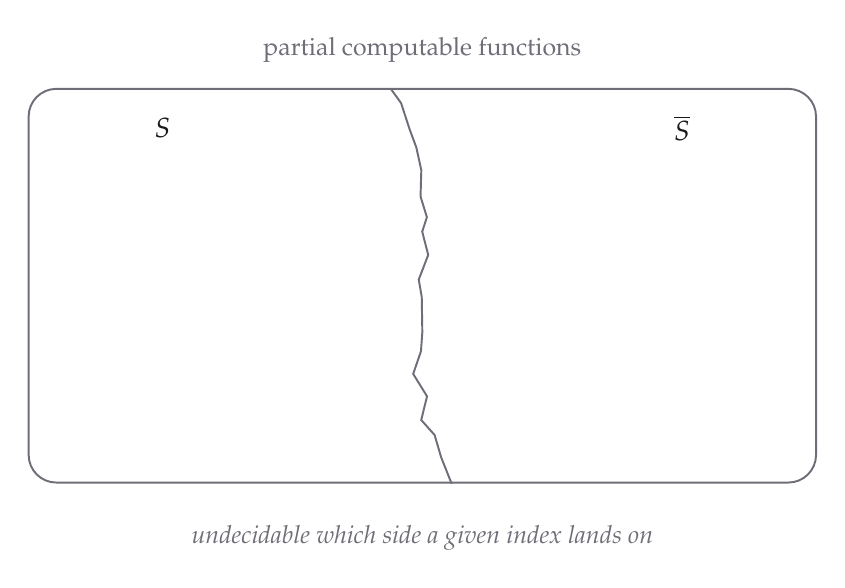
\begin{tikzpicture}[scale=1.0]
    % Universe blob
    \node[space_blob, minimum width=10cm, minimum height=5cm] (univ) at (0,0) {};
    % Wavy divider
    \draw[space_divide] (-0.4, 2.5) .. controls (0.6, 1) and (-0.6, -1) .. (0.4, -2.5);
    \node[figure_label] at (-3.3, 2.0) {$S$};
    \node[figure_label] at (3.3, 2.0) {$\overline{S}$};
    \node[figure_label, text=color_mute, font=\rmfamily\itshape\small]
      at (0, -3.2) {undecidable which side a given index lands on};
    \node[figure_label, font=\rmfamily\small, text=color_mute]
      at (0, 3.0) {partial computable functions};
  \end{tikzpicture}
\end{frame}

\begin{frame}{Rice's theorem, proof}
  \small
  \begin{itemize}
    \item Pick $a, b \in \N$ with $a \in S$ and $b \notin S$.
    \item Define $f(e, x)$ by cases:
      \begin{itemize}
        \item $f(e, x) = \varphi_b(x)$ when $e \in S$
        \item $f(e, x) = \varphi_a(x)$ when $e \notin S$
      \end{itemize}
    \item By s-m-n, there is $e$ with $\varphi_e(x) = f(e, x)$.
    \item If $e \in S$ then $\varphi_e = \varphi_b$, but $b \notin S$.
    \item If $e \notin S$ then $\varphi_e = \varphi_a$, but $a \in S$.
    \item Either way: contradiction. \hfill$\square$
  \end{itemize}
\end{frame}

\begin{frame}{Rice's theorem, as a diagram}
  \centering
  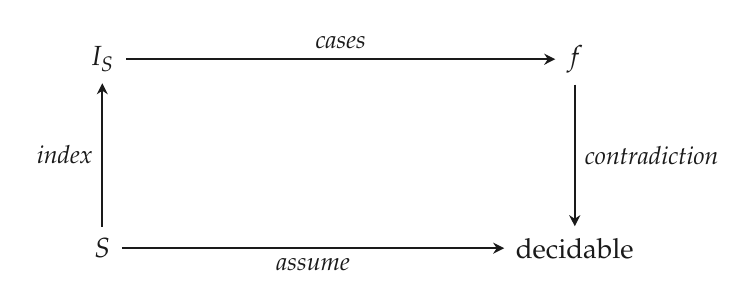
\begin{tikzpicture}[node distance=3.6cm and 5.0cm]
    \node[diagram_node] (IS)   at (0, 2.4)  {$\IS$};
    \node[diagram_node] (f)    at (6, 2.4)  {$f$};
    \node[diagram_node] (S)    at (0, 0)    {$S$};
    \node[diagram_node] (dec)  at (6, 0)    {decidable};

    \draw[diagram_arrow] (S) -- (IS) node[midway, left, figure_label, font=\rmfamily\itshape\small] {index};
    \draw[diagram_arrow] (IS) -- (f) node[midway, above, figure_label, font=\rmfamily\itshape\small] {cases};
    \draw[diagram_arrow] (S) -- (dec) node[midway, below, figure_label, font=\rmfamily\itshape\small] {assume};
    \draw[diagram_arrow] (f) -- (dec) node[midway, right, figure_label, font=\rmfamily\itshape\small] {contradiction};
  \end{tikzpicture}
  \vskip 1em
  {\small\itshape\color{color_mute} Same proof, drawn as a fixed-point square.}
\end{frame}

\begin{frame}{Rice's theorem, contrapositive}
  \begin{block}{}
    If $\IS$ is decidable, then $S$ is trivial.
  \end{block}
  \vskip 0.7em
  The only decidable function properties are no property at all.
\end{frame}

%%%---- Rice-Shapiro
\begin{frame}{Rice--Shapiro}
  \begin{itemize}
    \item \emph{Rice.} If $S$ is non-trivial, then $\IS$ is undecidable.
    \item \emph{Shapiro.} $f \in S \iff \exists\, \text{finite } g \subseteq f \text{ with } g \in S$.
  \end{itemize}
  \vskip 0.6em
  {\small\itshape\color{color_mute}
   The word that earns its keep here is \emph{finite}.}
\end{frame}

\begin{frame}{Rice--Shapiro, the witness}
  \centering
  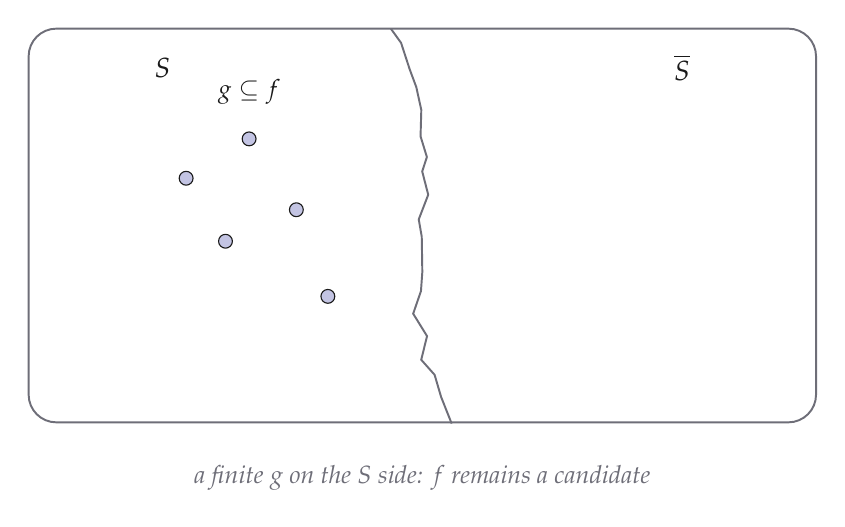
\begin{tikzpicture}[scale=1.0]
    \node[space_blob, minimum width=10cm, minimum height=5cm] (univ) at (0,0) {};
    \draw[space_divide] (-0.4, 2.5) .. controls (0.6, 1) and (-0.6, -1) .. (0.4, -2.5);
    \node[figure_label] at (-3.3, 2.0) {$S$};
    \node[figure_label] at (3.3, 2.0) {$\overline{S}$};
    % Candidate f cloud on left
    \node[witness_dot] (g1) at (-3.0, 0.6) {};
    \node[witness_dot] (g2) at (-2.2, 1.1) {};
    \node[witness_dot] (g3) at (-2.5, -0.2) {};
    \node[witness_dot] (g4) at (-1.6, 0.2) {};
    \node[witness_dot] (g5) at (-1.2, -0.9) {};
    \node[figure_label, font=\rmfamily\itshape\small] at (-2.2, 1.7) {$g \subseteq f$};
    \node[figure_label, text=color_mute, font=\rmfamily\itshape\small]
      at (0, -3.2) {a finite $g$ on the $S$ side: $f$ remains a candidate};
  \end{tikzpicture}
\end{frame}

\begin{frame}{Rice--Shapiro, the refutation}
  \centering
  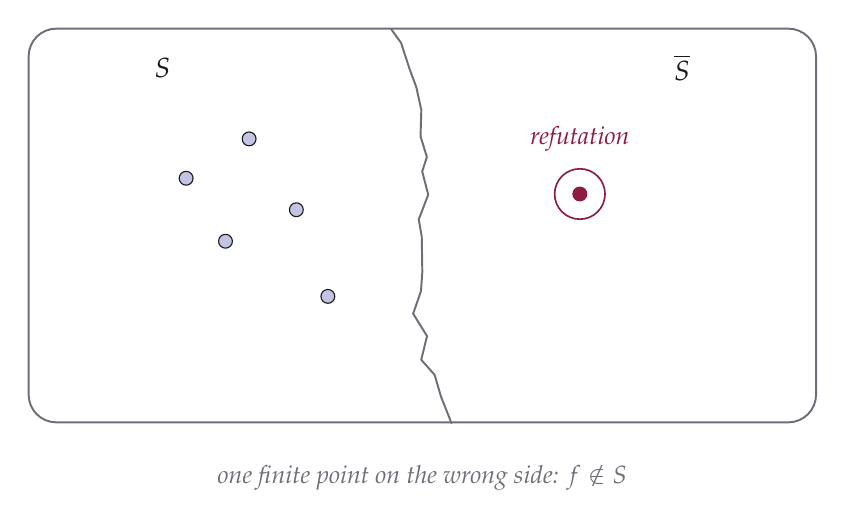
\begin{tikzpicture}[scale=1.0]
    \node[space_blob, minimum width=10cm, minimum height=5cm] (univ) at (0,0) {};
    \draw[space_divide] (-0.4, 2.5) .. controls (0.6, 1) and (-0.6, -1) .. (0.4, -2.5);
    \node[figure_label] at (-3.3, 2.0) {$S$};
    \node[figure_label] at (3.3, 2.0) {$\overline{S}$};
    \node[witness_dot] (g1) at (-3.0, 0.6) {};
    \node[witness_dot] (g2) at (-2.2, 1.1) {};
    \node[witness_dot] (g3) at (-2.5, -0.2) {};
    \node[witness_dot] (g4) at (-1.6, 0.2) {};
    \node[witness_dot] (g5) at (-1.2, -0.9) {};
    % The refuting point
    \node[refutation_dot] (gx) at (2.0, 0.4) {};
    \draw[color_accent, line width=0.6pt] (gx) circle (0.32cm);
    \node[figure_label, text=color_accent, font=\rmfamily\itshape\small]
      at (2.0, 1.1) {refutation};
    \node[figure_label, text=color_mute, font=\rmfamily\itshape\small]
      at (0, -3.2) {one finite point on the wrong side: $f \notin S$};
  \end{tikzpicture}
\end{frame}

\begin{frame}{Rice--Shapiro, proof}
  \vfill
  \centering
  {\large\itshape\color{color_mute} sketch to come}
  \vfill
\end{frame}

\begin{frame}{Rice--Shapiro, as a diagram}
  \vfill
  \centering
  {\large\itshape\color{color_mute} category-theory diagram to come}
  \vfill
\end{frame}

\begin{frame}{Rice--Shapiro, contrapositive}
  \begin{itemize}
    \item If $g \in S$ and some finite $h \subseteq g$ has $h \notin S$, then $\IS$ is not \re
    \item The witness can refute, not just confirm.
  \end{itemize}
\end{frame}

\begin{frame}{Plain English, all four}
  \begin{itemize}
    \item \emph{Rice.} Non-trivial behavioral properties are undecidable.
    \item \emph{Rice, contrapositive.} Decidable means trivial.
    \item \emph{Rice--Shapiro.} Behavior is fixed by finite evidence.
    \item \emph{Rice--Shapiro, contrapositive.} One finite witness against you, and the index set is not even \re
  \end{itemize}
\end{frame}

\begin{frame}{Bridge to history}
  \begin{itemize}
    \item Rice--Shapiro: one counterexample is enough.
    \item Mathematicians arrived here in 1956.
    \item The rest of the scientific world had been working on it for a while.
  \end{itemize}
  \vskip 0.6em
  {\small\itshape\color{color_mute} Let's talk some history.}
\end{frame}

\end{document}
